\documentclass[portrait, a1paper, fontscale=0.5]{baposter}

\usepackage[utf8]{inputenc}
\usepackage{graphicx}

\definecolor{bgcolorone}{RGB}{225,225,225}
\definecolor{bgcolortwo}{RGB}{225,225,225}
\definecolor{bordercolor}{RGB}{153,153,153}
\definecolor{headercolorone}{RGB}{255,255,255}
\definecolor{headercolortwo}{RGB}{255,255,255}
\definecolor{headerfontcolor}{RGB}{7,67,145}
\definecolor{boxcolorone}{RGB}{200,200,200}

\pdfinfo
{
	/Title (SNA)
	/Author (P. Kus, P. Karban, F. Mach)
}

\begin{document}

\background{}

\begin{poster}{
	grid=false,
	columns=6,
	background=plain,
	bgColorOne=bgcolorone,
	%bgColorTwo=bgcolortwo,
	borderColor=bordercolor,
	headerColorOne=headercolorone,
	headerColorTwo=headercolortwo,
	headerFontColor=headerfontcolor,
	boxColorOne=boxcolorone,
	headershape=roundedright,
	headerfont=\large\sc,
	textborder=roundedleft,
	background=user,
	headerborder=open,
	boxshade=none
}
{
\includegraphics[width=17em]{fel.pdf}}
{\huge\textsc{\textcolor{headerfontcolor}{Solving nonlinear coupled problems using Agros2D}}\vspace{0.75em}}
{\Large{\textcolor{headerfontcolor}{P. Kus$^{1}$, P. Karban$^{2}$ and F. Mach$^{1, 2}$\\{\large $^{1}$ \textit{Institute of Thermomechanics, Academy of Sciences CR, v. v. i.}}\\{\large $^{2}$ \textit{Faculty of Electrical Engineering, University of West Bohemia}}}}}
{
\includegraphics[width=7em]{it.png}}

\headerbox{About Agros2D}{name=about,column=0,row=0, span=2}{
Agros2D is a multiplatform C++ application for the solution of partial differential equations (PDE) based on the Hermes library, developed by the hpfem.org group at the University of West Bohemia in Pilsen. Hermes library is developed at University od Reno in Nevada. Agros2D is distributed under the GNU General Public License.
}

\headerbox{Supported physical fields}{name=fields,column=0,row=0, span=2,below=about}{
\begin{itemize} \itemsep1pt \parskip0pt \parsep0pt
\item Electrostatic fields
\item Electric current fields
\item Magnetic fields (steady state, harmonic and transient analysis)
\item High frequency electromagnetic fields - in development
\item Temperature fields (steady state and transient)
\item Acoustic field (harmonic and transient analysis)
\item Linear thermo-elasticity
\item Incompressible flow  - in development
\end{itemize}
}

\headerbox{Key Features}{name=features,column=0,row=0,span=2,below=fields}{
\begin{itemize} \itemsep1pt \parskip0pt \parsep0pt
\item Steady state, transient and harmonic analysis
\item Curvilinear elements
\item Arbitrary level hanging nodes
\item Multimesh assembling
\item Automatic hp-adaptivity
\end{itemize}
}

\headerbox{Simple GUI control}{name=gui,column=0,row=0,span=2,below=features}{
\begin{itemize} \itemsep1pt \parskip0pt \parsep0pt
\item Interactive geometry definition
\item AutoCAD DXF (Drawing Exchange Format) import and export
\item Visualization of field variables
\item Extraction of local values
\item Calculation of surface and volume integrals
\item Export of charts, data, and images
\item Export movies (transient analysis)
\item Scripting support (based on Python language)
\item Remote control
\end{itemize}
}

\headerbox{Adaptivity}{name=adaptivity ,column=0,row=0,span=2,below=gui}{
\begin{center}
	\begin{minipage}{22em}
		One of the main strengths of the Hermes library, which is also available in Agros2D, is an automatic
$hp$-adaptivity algorithm. It combines advantages of $h$-adaptivity (precise resolution of singularities, 
boundary layers, etc.) with advantages of $p$-adaptivity, which is very successfull for smooth solutions. 
Its superiority can bee seen from the following graph, where different adaptivity strategies are compared 
for test problem.
\end{minipage}
\begin{minipage}{22em}
\hspace{-0.7cm}
	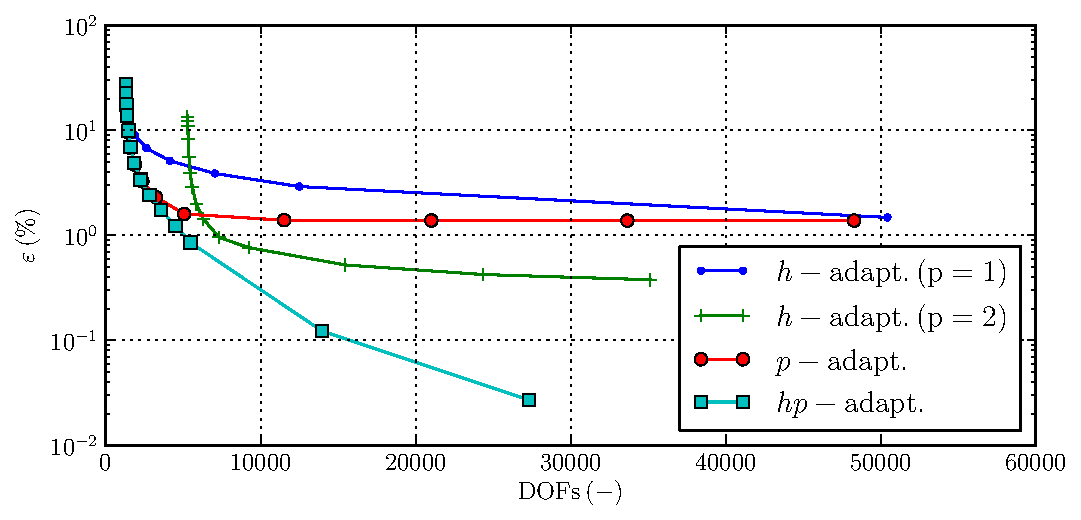
\includegraphics[width=24em]{adaptivity/convergence.pdf}
	\end{minipage}
\end{center}
}

\headerbox{Curvilinear elements}{name=curvilinear_elements,column=0,row=0,span=3,below=adaptivity}{
\begin{center}
	\begin{minipage}{19em}
		\centering
		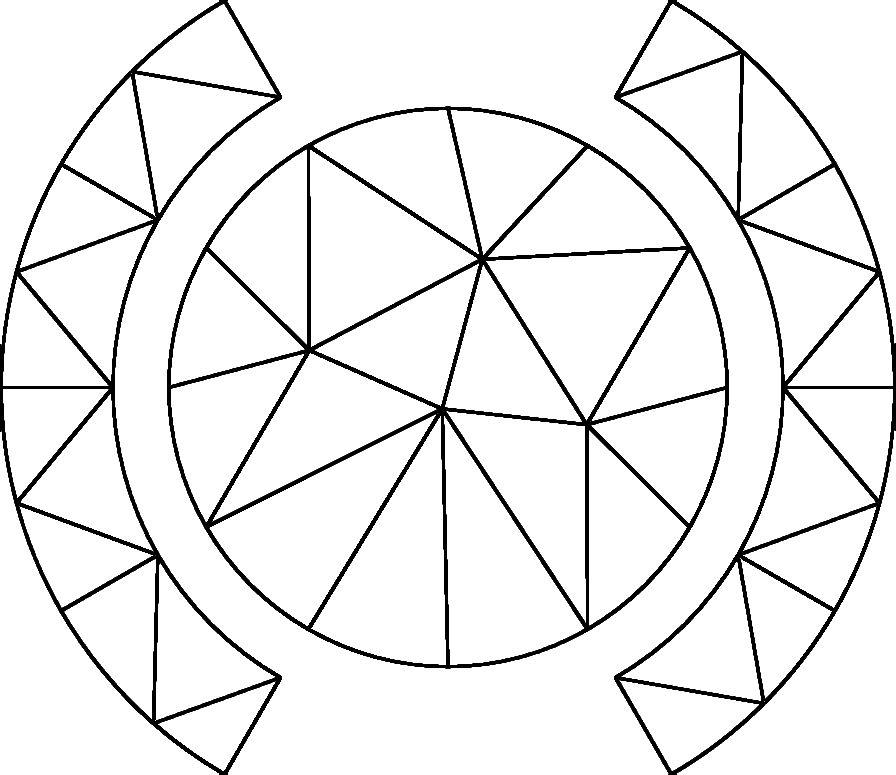
\includegraphics[angle=90, width=19em]{curvilinear_elements/mesh.png}
	\end{minipage}
\begin{minipage}{19em}
The use of curvilinear elements can be very effective for some geometries. In the classical approach, 
rounded lines have to be approximated by a sequence of small streight segments. 
In the figure left we can see part of insulator and its mesh.
It would result in loss of 
accuracy and also in creation of large amount of elements in the initial mesh. The use of curvilinear 
elements hence leads to faster and more accurate calculations.
\end{minipage}

\end{center}}

\headerbox{Arbitrary level hanging nodes}{name=arbitrary,column=3,row=0,span=3,below=adaptivity}{
\begin{center}
	\begin{minipage}{20em}
		\centering
		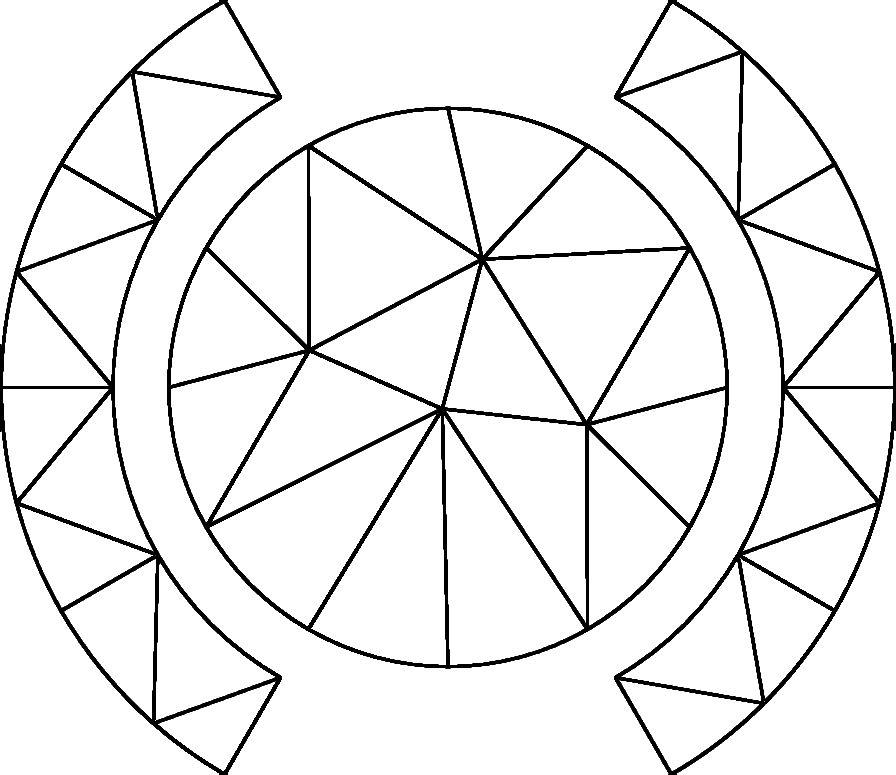
\includegraphics[angle=90, width=19em]{curvilinear_elements/mesh.png}
	\end{minipage}
\begin{minipage}{17em}
Use of meshes with arbitrary-level hanging nodes with higher-order approximation is a unique feature of 
the Hermes library. In connection with automatic adaptivity, it allowes to resolve difficoult problems 
precisely. An example of such mesh can be seen in the figure left.
\end{minipage}

\end{center}}

\headerbox{Optimization}{name=optimization,column=2,row=0,span=4}{
\begin{center}
        \begin{minipage}{16.5em}
	    In the engineering practise, the usual demand is not only to calculate some field, 
	    but also to be able to design some of the construction parameters in order to 
optimize some properties. In Agros2D, optimization is possible thanks to scripting -- a python 
interpreter is included.
	\end{minipage}
	\begin{minipage}{4em}
		\centering
		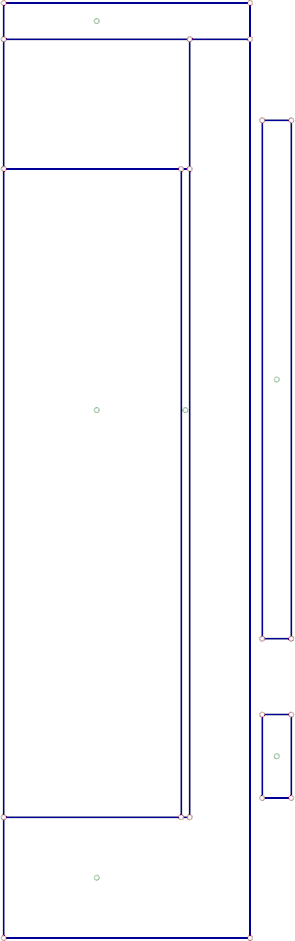
\includegraphics[scale=0.125]{optimization/variant_1.png}
	\end{minipage}
	\begin{minipage}{10em}
		\centering
		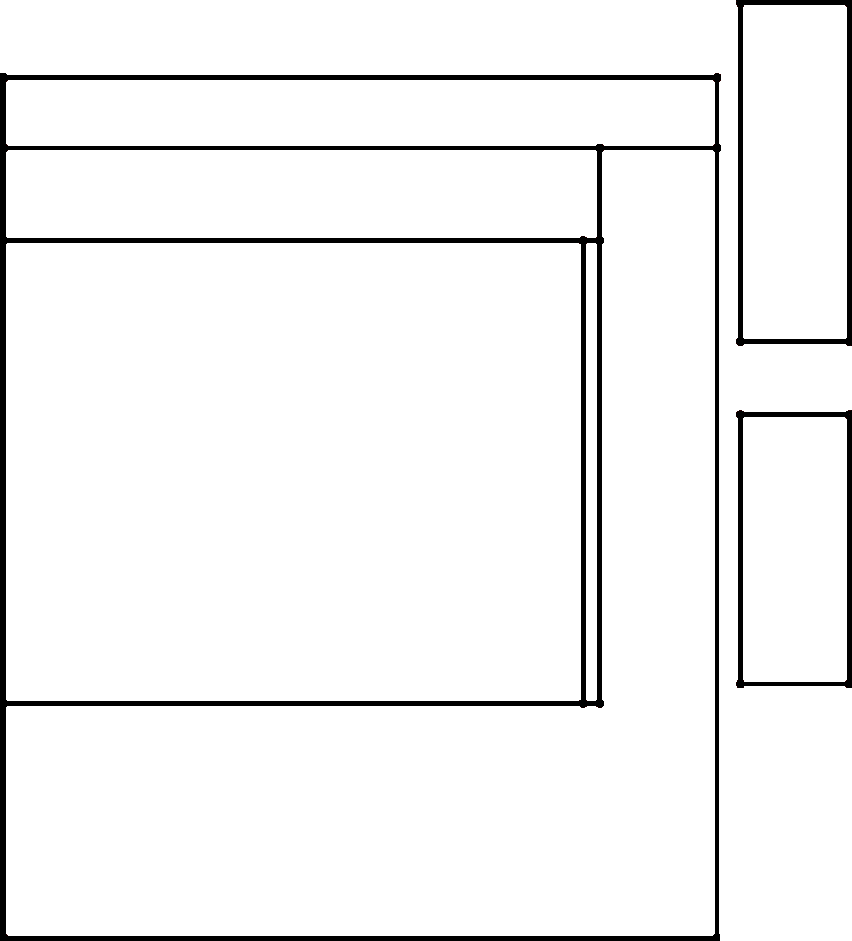
\includegraphics[scale=0.125]{optimization/variant_2.png}
	\end{minipage}
	\begin{minipage}{8em}
		\centering
		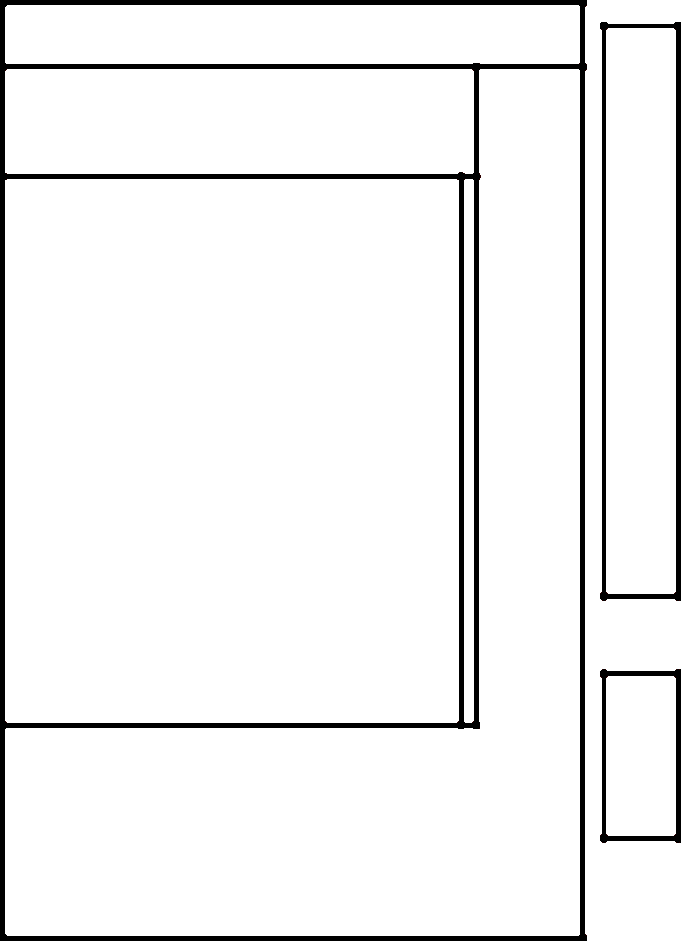
\includegraphics[scale=0.125]{optimization/variant_3.png}
	\end{minipage}
	\begin{minipage}{10em}
		\centering
		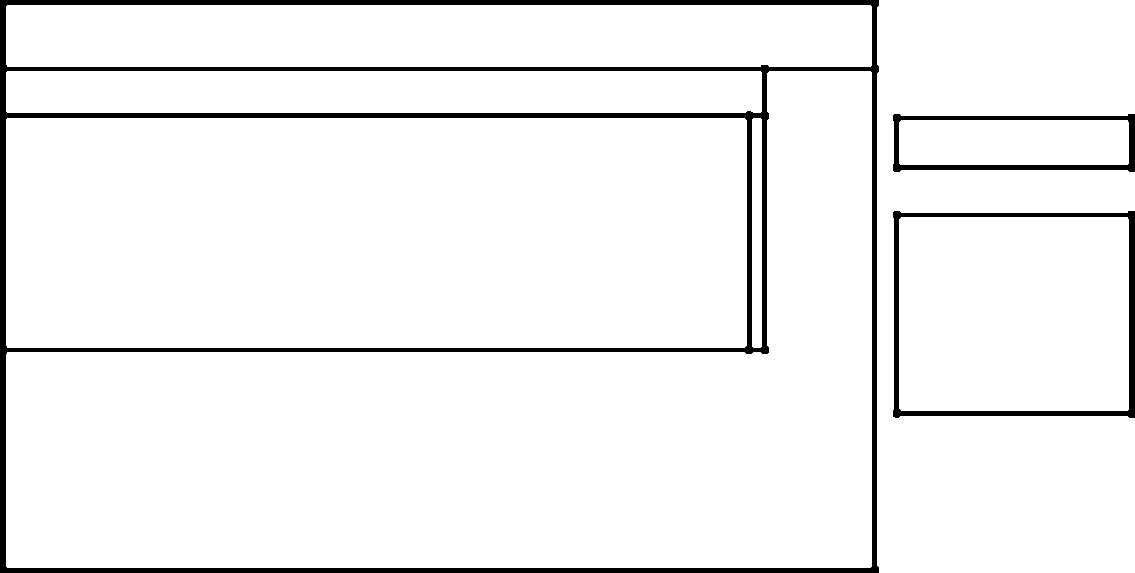
\includegraphics[scale=0.105]{optimization/variant_4.png}
	\end{minipage}
\end{center}

\begin{center}
	\begin{minipage}{12em}
		\centering
		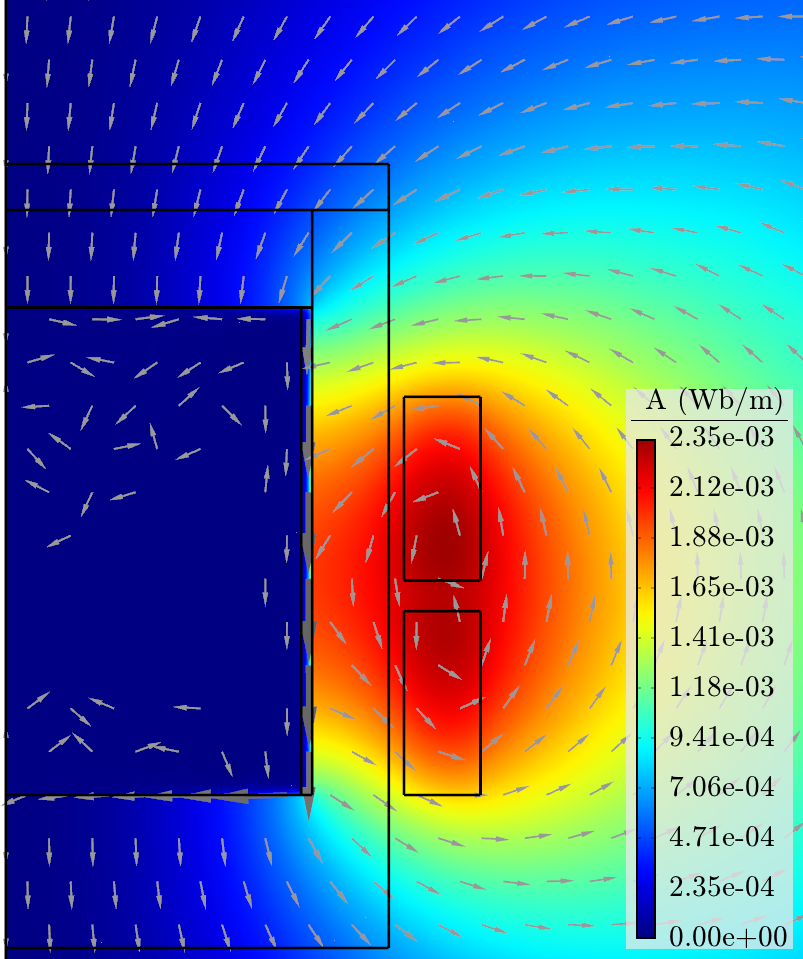
\includegraphics[height=14em]{optimization/magnetic_field.png}
	\end{minipage}
	\begin{minipage}{12em}
		\centering
		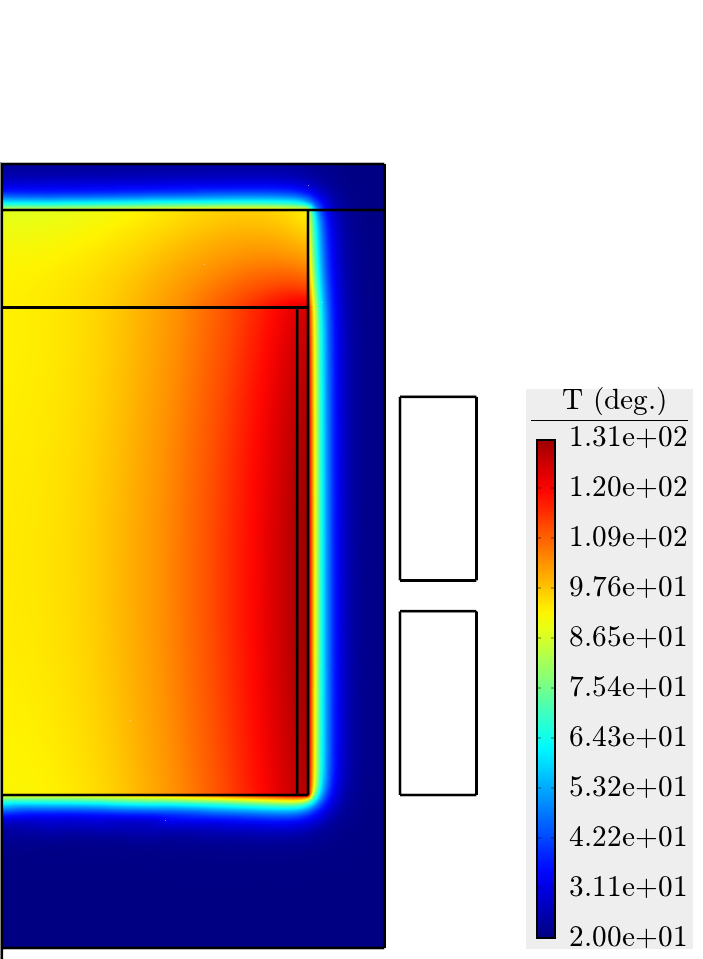
\includegraphics[height=14em]{optimization/temperature_field.png}
	\end{minipage}
	\begin{minipage}{24em}
		In the figure above, we can see several configurations of an owen used for induction heating.
The schema (and also the calculations) are axisymetric.
Several parameters can be changed -- the shape of the owen (height and diameter) can changed, but its volume remains constant.
Also the position and size of inductors (two bars on the right hand side of the figure) can be changed. In the figure left we can 
see magnetic field generated by the inductor and temperature field generated by Joule losses in the material.
	\end{minipage}
\end{center}

\begin{center}
	\begin{minipage}{25em}
		In this problem, there are two different indicators of the quality of the design. First, total heat generated in the 
owen should be as big as possible, and, second, it should be equaly distributed. In the figure, each point represents one calculation 
and its resulting heat $Q$ (should be maximalized) and unevennes of distribution of heat $U$ (shoul be minimalized). Blue points represent
calculations with randomly chosen parameters. Red points are products of optimization (simple implementation of conjugate gradient method has
been used). ...
	\end{minipage}
	\begin{minipage}{25em}
		\centering
		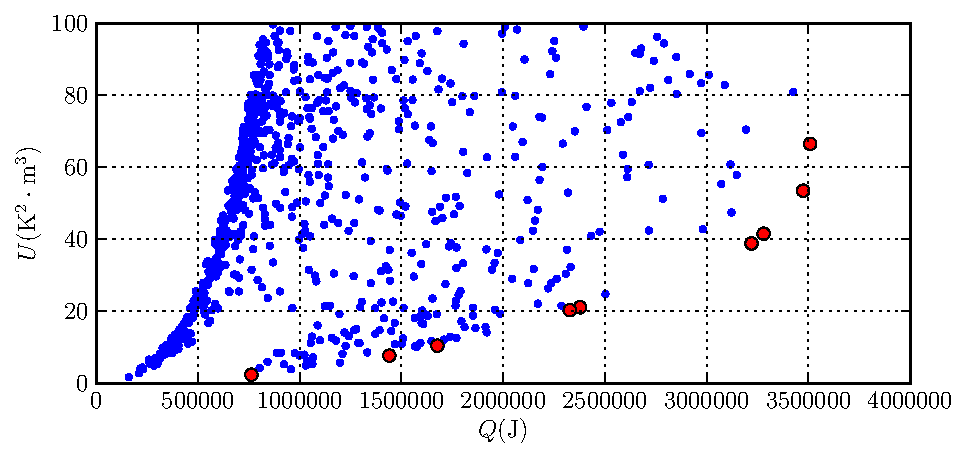
\includegraphics[width=25em]{optimization/results.pdf}
	\end{minipage}
\end{center}
}

\headerbox{Particle tracing}{name=particle_tracing,column=2,row=0,span=4,below=optimization}{
\begin{center}
	\begin{minipage}{17.5em}
		Particle tracing is a feature, that has been addede to Agros2D just recently. It calculates how charged particle 
behave in calculated field. We demonstrate this feature on an example of device, which is used for separation of
different components of recycled material. A schema of such separator is shown in the figure right.
	\end{minipage}
	\begin{minipage}{15em}
			\centering
	 		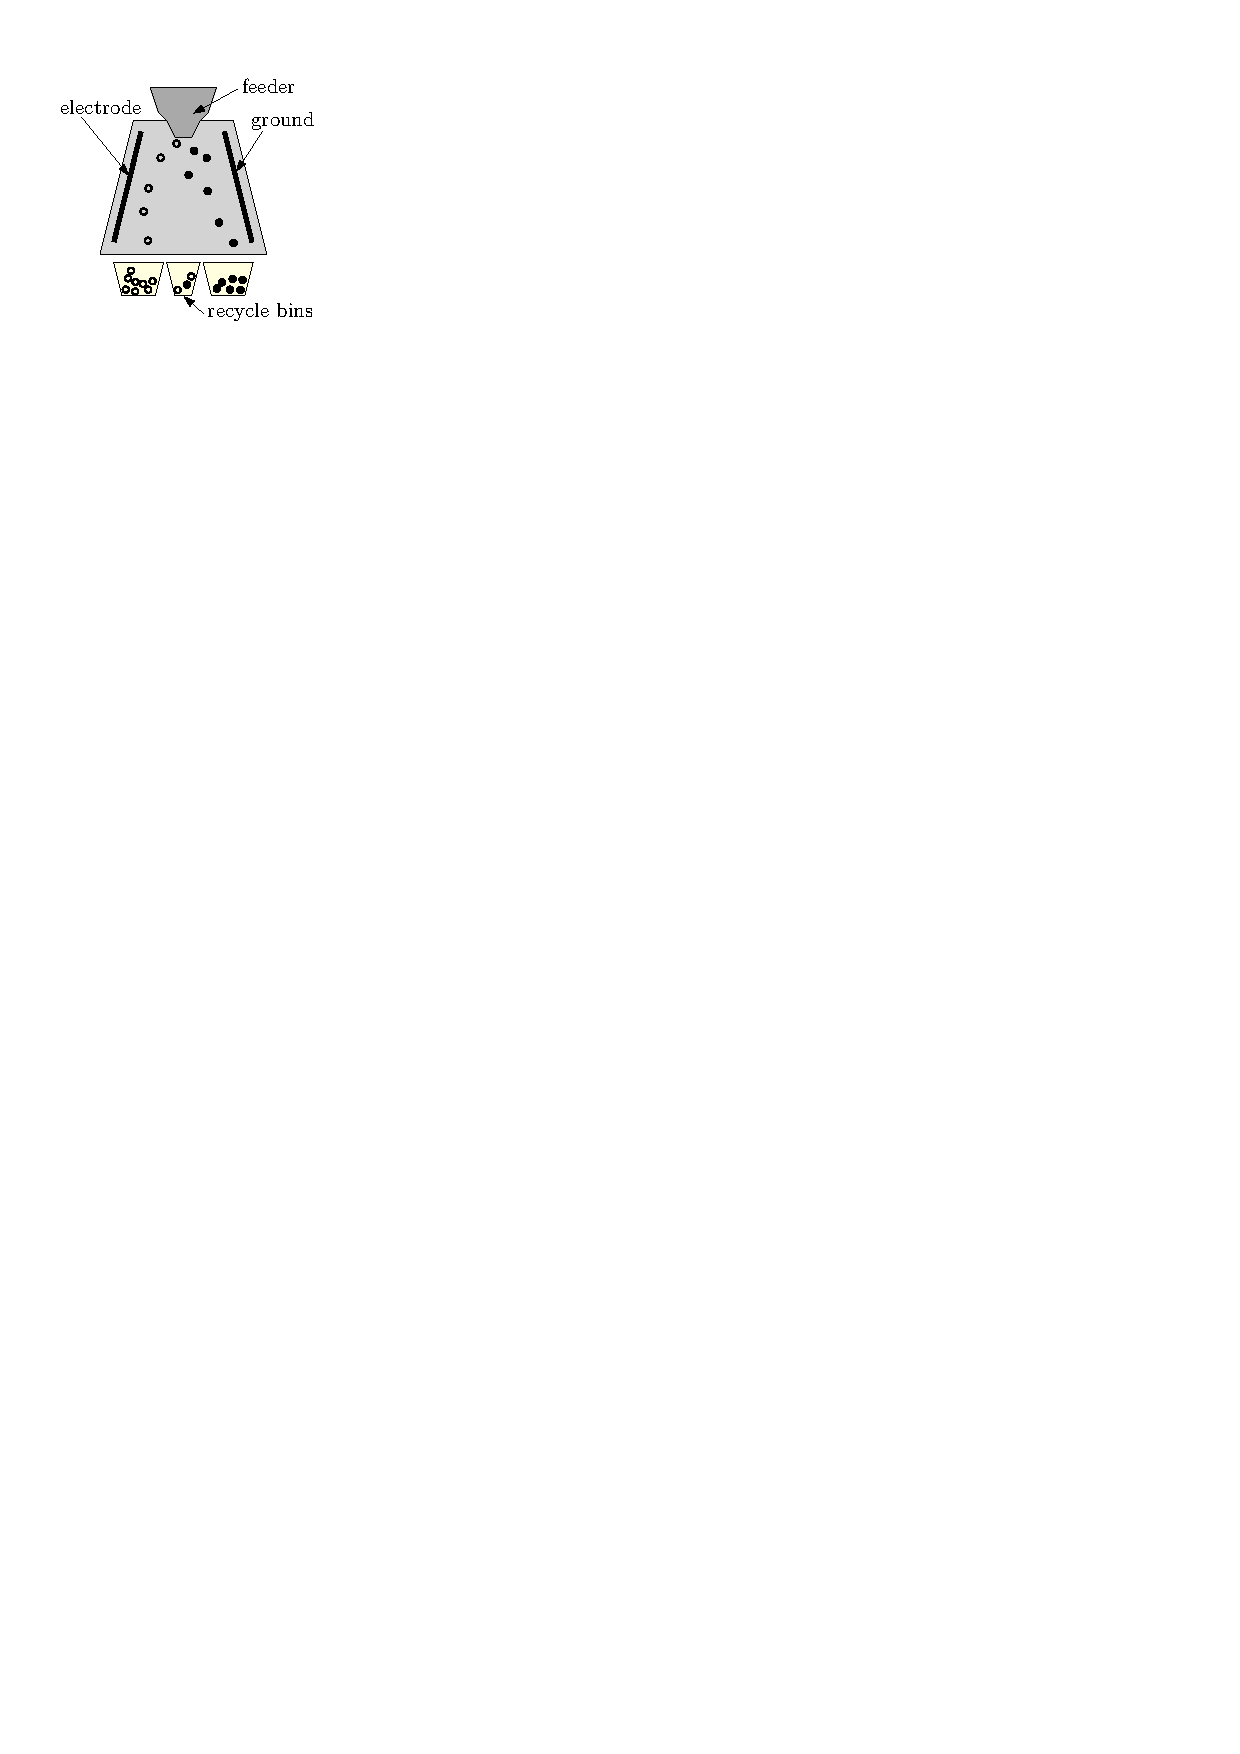
\includegraphics{particle_tracing/principle.pdf}
	\end{minipage}
  \begin{minipage}{17.5em}
Electric field potential is calculated first. $hp$-adaptivity has been used, since it is very efficient for 
electorstatic problems. In the figure below we can see fine mesh, that has been created by automatic adaptivity
algorithm. It can be seen, that the mesh is very fine close to the singularities of the field and that various
polynomial degrees are used, as it is optimal to minimize the solution error.
  \end{minipage}
\end{center}

\begin{center}
	\begin{minipage}{20em}
		\centering
	 	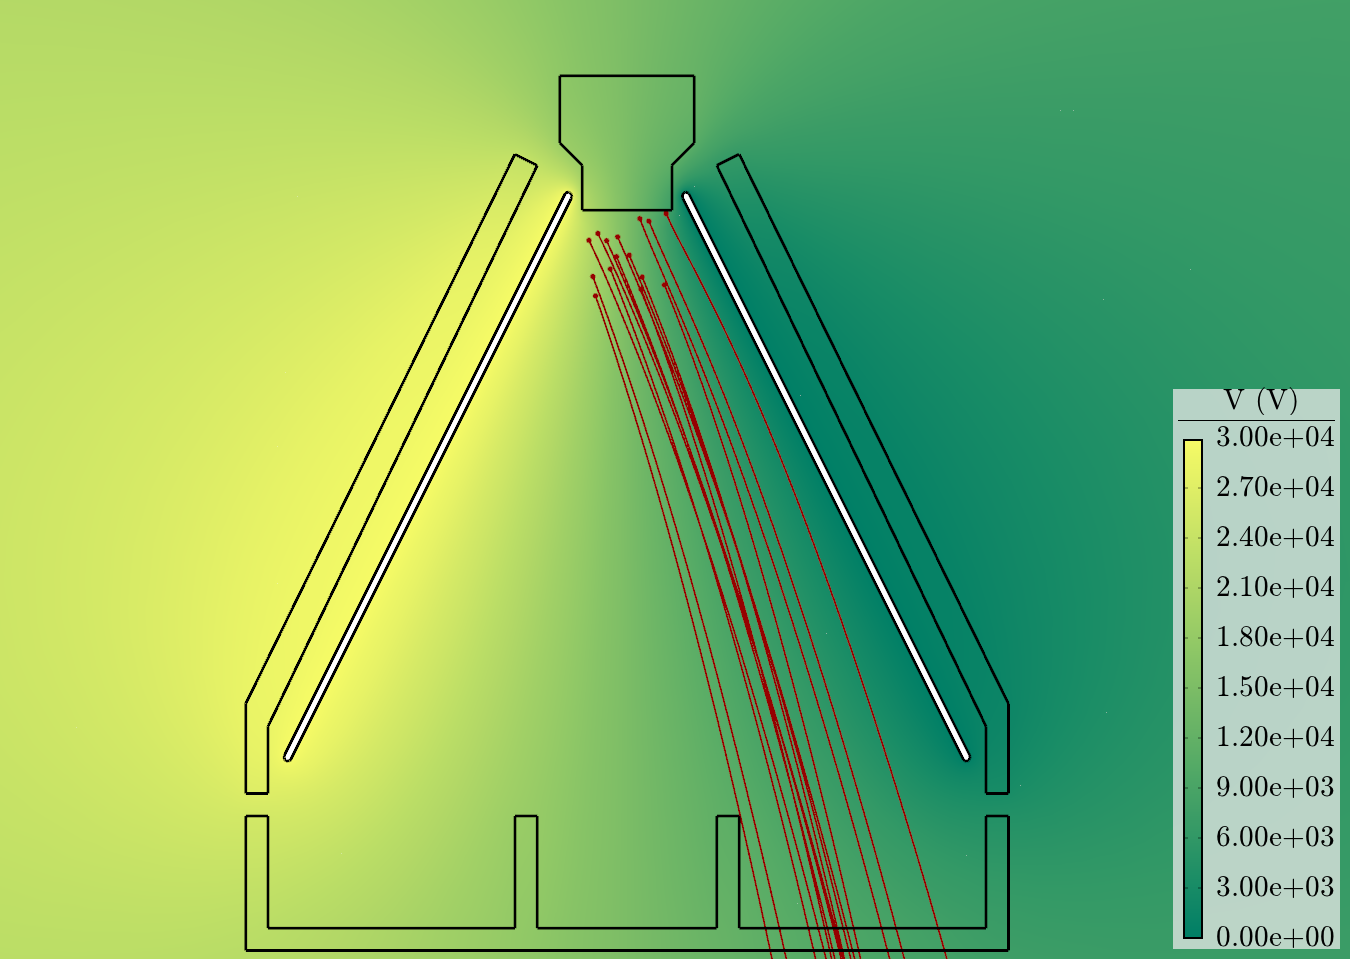
\includegraphics[width=19em]{particle_tracing/scalar_potential_and_particles.png}
	\end{minipage} 
	\begin{minipage}{11em}
		In the figure left we can see electric potential and traces of several particles, as they are directed to 
right container of the separator. Electric field acts differently for each type of particles, which is the 
principle of separation.
	\end{minipage}
	\begin{minipage}{20em}
		\centering
	 	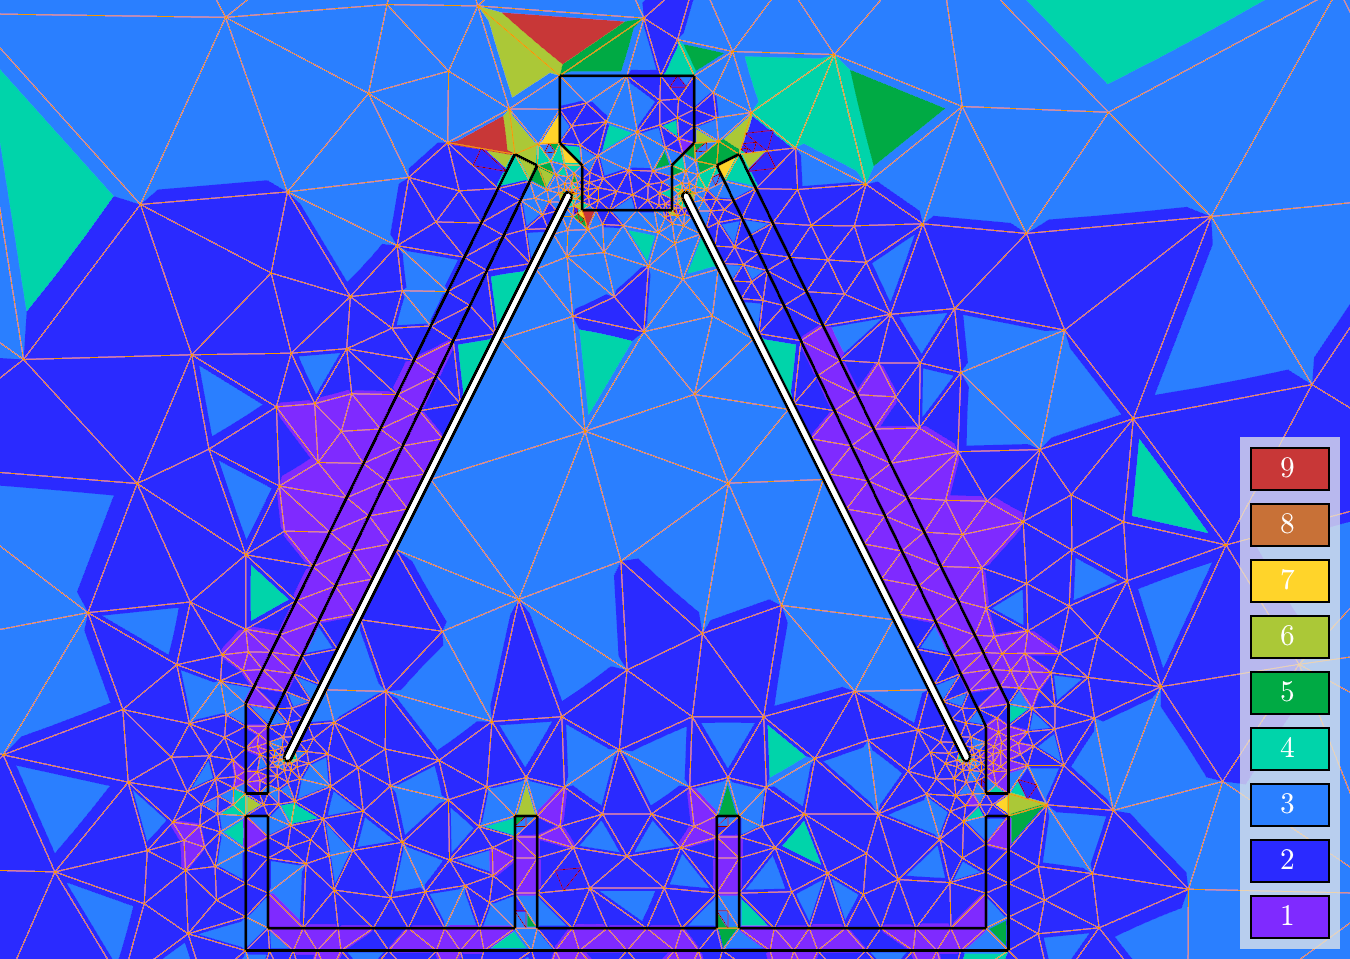
\includegraphics[width=19em]{particle_tracing/mesh_and_polynomial_order.png}
	\end{minipage} 
\end{center}

}
\headerbox{References}{name=references,column=0,row=0,span=6,below=particle_tracing, below=curvilinear_elements}{
}
\end{poster}
\end{document}